\documentclass[10pt,a4paper]{article}
\usepackage[utf8x]{inputenc}
\usepackage{ucs}
\usepackage{amsmath}
\usepackage{amsfonts}
\usepackage{amssymb}
\usepackage{hyperref}
\usepackage{graphicx}
\usepackage{float}
\usepackage{listings}
\lstset{language=bash,basicstyle=\footnotesize}%, numbers=left}


\author{Olaf Radicke}
\title{Dokumentation der Funktionsweise der OSR-Dracut-Module}


\begin{document}

\maketitle

\newpage 

\tableofcontents

\newpage 

\section{Gernerell}

Als erstes wird vom Kernel nach dem Booten ein kleiner Binär-Code von Dracut ausgeführt, der dann seinerseits die in dash geschriebene Dracut-Module ausführt. Das erste Modul das von Darcut startet wird ist das Modul 99base. Das Erste was das Modul tut ist, dafür zu sorgen das dass initramfs geladen hat. Das Script was dafür verantwortlich ist, ist die \texttt{init}-Datei. Diese kann angepasst werden. Empfohlen wird aber stat dessen die Hooks zu verwenden. Hooks sind Scrips die vor oder nach definierten Ereignissen ausgeführt werden. Diese Hooks werden in den Modulen in den Dateien \texttt{install} definiert.

\subsection{Verwendete Hooks}

Die in den Modulen verwendeten Hooks sind:
\begin{description}
 \item[cmdline] Ein sehr früher Zeitpunkt. Hier werden die Kerne-Parameter ausgewertet werden die dem Bootloader mitgegeben wurden (Sei es als GRUB-Konfiguration oder beim Booten). Hier werden z.B. die wichtigsten Environment-Variablen gesetzt. 
 \item[pre-pivot] Das ist der letzte Hook der ausgeführt wird, bevor  das richtige root-Verzeichnis ein gehangen wird. Also ein guter Zeitpunkt für etweilige Aufräumarbeiten.
\end{description}
 
\subsection{Verwendete undokumentierte Hooks}

Die volgenen Hooks ist in der Dracut-Doku nicht dokumentiert. Werden aber verwendet.

\begin{description}
 \item[emergency] 
 \item[netroot]
\end{description}

In einem Script \texttt{check} wird eine Funktion \texttt{check()} definiert. Das Scrip \texttt{check} sollte 0 (null) zurückgeben, wenn alle Bedingungen erfüllt sind. Wird ein anderer Wert zurückgegeben, wird das Modul nicht von Darcut geladen.

\subsection{Weitere Schlüsselworte (Methoden) von Dracut}

\begin{description}
 \item[inst\_simple] Mit dem Schlüsselwort \texttt{inst\_simple} werden Dateien in das initramfs kopiert/installiert.
 \item[dracut\_install] Mit dem Schlüsselwort \texttt{dracut\_install} werden Software-Pakete in die ramsf-Umgebung installiert bzw. zur Verfügung gestellt.
 \end{description}
 
\subsection{Verwendete Darcut-Lib-Komandos}

Die Dracut-lib (\texttt{/usr/share/dracut/modules.d/99base/dracut-lib.sh}) stellt verschiedene Methoden zur Verfühgung. Benutzt werden von OSR:

\begin{description}
 \item [getarg()] Gibt die benutzten Kernel-Parameter zurück.
 \item [die()] Schreibt eine Meldung in \texttt{/dev/kmsg}, gibt eine Meldung auf der Standartausgabe aus und beendet das Script mit Rückgabelwert 1.
 \item [info()] Schreibt Meldungen in  \texttt{/dev/kmsg}, mit die Informationen später, nach dem Booten vom Benutzer abgerufen werden können.

\end{description}

\subsection{Undokumentierte Dracut-Schnittstellen}

Handler für den netroot-Typ ( \texttt{/usr/share/dracut/modules.d/40network/netroot} ):
\begin{lstlisting}
# Check: do we really know how to handle (net)root?
[ -z "$root" ] && die "No or empty root= argument"
[ -z "$rootok" ] && die "Don't know how to handle 'root=$root'"

handler=${netroot%%:*}
handler=${handler%%4}
handler="/sbin/${handler}root"
if [ -z "$netroot" ] || [ ! -e "$handler" ] ; then
    die "No handler for netroot type '$netroot'"
fi
\end{lstlisting}

\textbf{/modules.d/95osr-cluster/osr-detect-root.sh }:

\begin{lstlisting}
if [ -z "$oldroot" ] || [ "$oldroot" = "autodetect" ]; then
    info "[osr-detect-root]: fstype: ${fstype} root: ${root} netroot: $netroot"
    # Network root scripts may need updated root= options,
    # so deposit them where they can see them (udev purges the env)
    {
        echo "root='$root'"
        echo "rflags='$rflags'"
        echo "fstype='$fstype'"
        echo "netroot='$netroot'"
        echo "NEWROOT='$NEWROOT'"
    } > /tmp/root.info
\end{lstlisting}

Bzw.: \texttt{/modules.d/95osr-cluster/install}

\begin{lstlisting}
inst "$moddir/osr-detect-root.sh" "/sbin/osr-detect-root"
inst "$moddir/osr-detect-root.sh" "/sbin/osrroot"
\end{lstlisting}

%%%%%%%%%%%%%%%%%%%%%%%%%%%%%%%%%%%%%%%%%%%%%%%%%%%%%%%%%%%%%%%%%%%%%%%%%%%%%%%%
% Die einzelen Module....
%%%%%%%%%%%%%%%%%%%%%%%%%%%%%%%%%%%%%%%%%%%%%%%%%%%%%%%%%%%%%%%%%%%%%%%%%%%%%%%%


%%%%%%%%%%%%%%%%%%%%%%%%%%%%%%%%% NEW SECTION %%%%%%%%%%%%%%%%%%%%%%%%%%%%%%%%%%
\section{Modul 95osr-chroot}

\subsection{Definierte Hooks}

\begin{tabular}{|l|l|l|}
 \hline
\textbf{Hook} & \textbf{Priorität} & \textbf{Script} \\ \hline
netroot  & 11 & osr-detect-chroot.sh \\ \hline
netroot  & 50 & osr-mount-chroot.sh \\ \hline
pre-udev & 51 & osr-move-chroot.sh \\ \hline
\end{tabular}

\subsubsection{osr-detect-chroot.sh}

Siehe \ref{osrdetectchroot} Seite \pageref{osrdetectchroot}.

\subsubsection{osr-mount-chroot.sh}

Siehe: \ref{osrmountchroot} Seite \pageref{osrmountchroot}.

\subsubsection{osr-move-chroot.sh}



%%%%%%%%%%%%%%%%%%%%%%%%%%%%%%%%% NEW SECTION %%%%%%%%%%%%%%%%%%%%%%%%%%%%%%%%%%

\section{Modul 95osr-cluster}

\subsection{Von Dracut zu installierende Software}

\begin{itemize}
 \item tr
 \item expr
 \item mkdir
 \item basename
\end{itemize}

\subsection{Definierte Hooks}

\begin{tabular}{|l|l|l|}
 \hline
\textbf{Hook} & \textbf{Priorität} & \textbf{Script} \\ \hline
pre-udev   & 59 & osr-net-genrules.sh \\ \hline
netroot    & 11 & osr-detect-chroot.sh \\ \hline
netroot    & 50 & osr-mount-chroot.sh \\ \hline
\end{tabular} 


\subsubsection{osr-net-genrules.sh}

\begin{description}
\item[Hook:] pre-udev
\item[Priorität:] 59
\end{description}

Das Script setzt die udev-Regeln.

\subsubsection{osr-detect-chroot.sh}
\label{osrdetectchroot} 

\begin{description}
\item[Hook:] netroot
\item[Priorität:] 11
\end{description}

Das Script überprüft, ob für den Node eine ID gesetzt ist. Wenn nicht bricht es mit einer Fehlermeldung ab. Ist die ID gesetzt wird \verb|/etc/conf.d/osr-nodeidvalues-${nodeid}.conf| eingebunden. Dann wird geprüft ob eine chroot-Umgebung gebraucht wird. Das Ergebnis der Prüfung wird gespeicherte mit \texttt{osr\_param\_store()}

\begin{figure}[H]
 \centering
 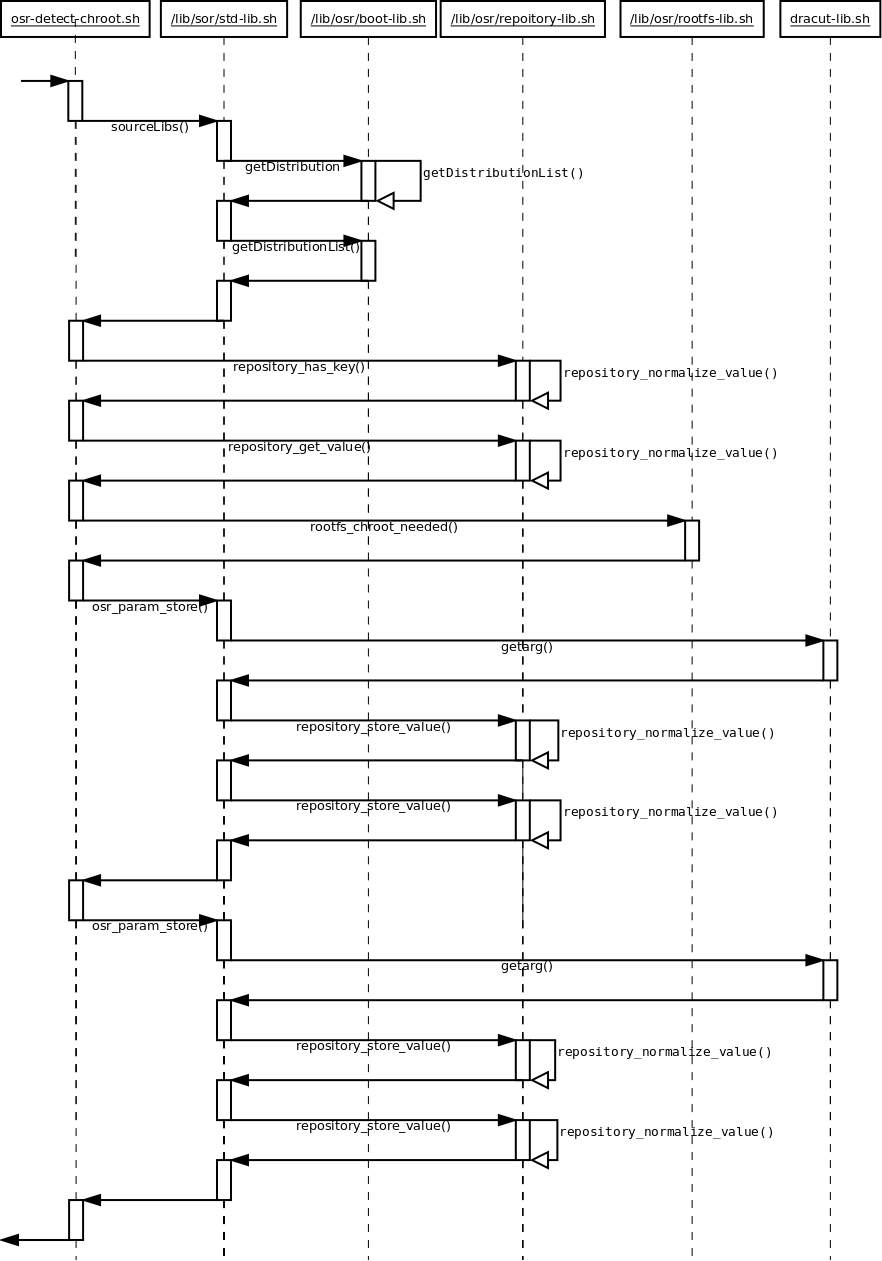
\includegraphics[width=1.0\textwidth,height=1.0\textwidth]{./sequence_diagram_osr-detect-chroot_DE_de.png}
 \caption[]{Sequence-Diagram des osr-detect-chroot.sh-Scrips}
\end{figure}

\subsubsection{osr-mount-chroot.sh}
\label{osrmountchroot} 

\begin{description}
\item[Hook:] netroot
\item[Priorität:] 50
\end{description}

Das Script hängt das richtige (shared) root-Verzeichnis ein. Schlägt das fehl, wird versucht das noch ein mal mit default Werten zu versuchen. Dann Werden die nötigen Ordnerstrukturen kopiert und die besonderen Verzeichnisse eingehangen.

\begin{verbatim}
  cp -axf $chroot_source $chroot_path
  rm -rf $chroot_path/var/run/*
  mkdir -p $chroot_path/tmp
  chmod 755 $chroot_path
  mount -t tmpfs none $chroot_path/dev
  cp -a /dev $chroot_path/
  mount -t devpts none $chroot_path/dev/pts
  mount -t proc proc $chroot_path/proc
  mount -t sysfs sysfs $chroot_path/sys
\end{verbatim}

\begin{figure}[H]
 \centering
 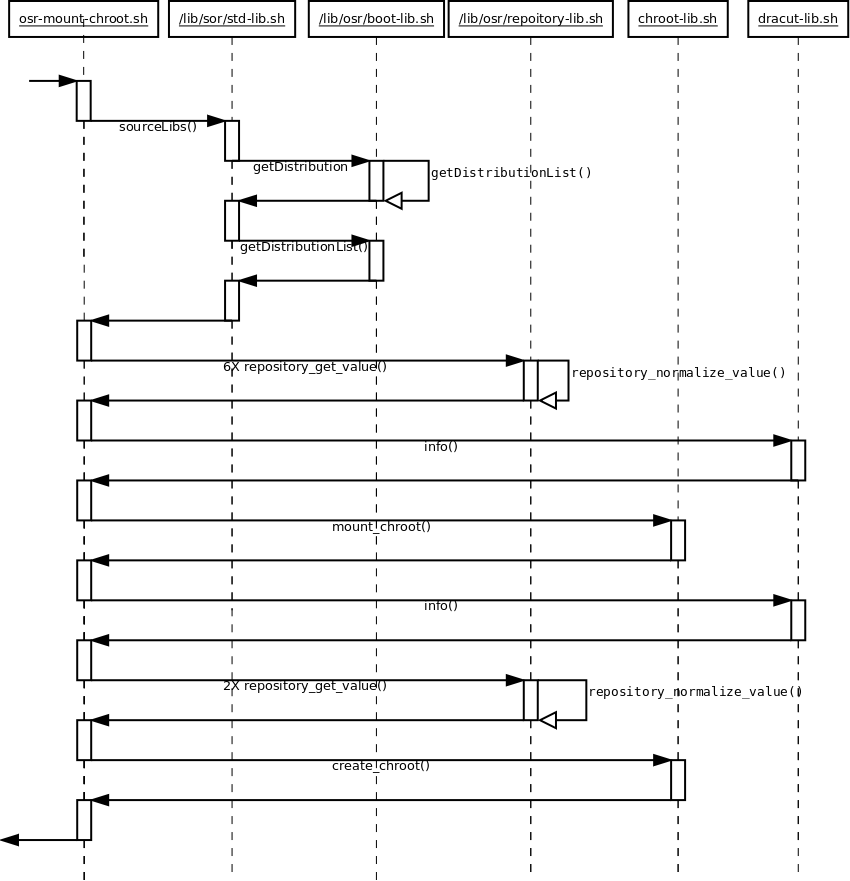
\includegraphics[width=1.0\textwidth,height=1.0\textwidth]{./sequence_diagram_osr-mount-chroot_DE_de.png}
 \caption[]{Sequence-Diagram des osr-mount-chroot.sh-Scrips}
\end{figure}


%%%%%%%%%%%%%%%%%%%%%%%%%%%%%%%%% NEW SECTION %%%%%%%%%%%%%%%%%%%%%%%%%%%%%%%%%%

\section{Modul 96osr}

Das Modul ist dafür zuständig, das File System für ein \texttt{shared root} ein zu hängen.

\subsection{In Initramfs installierte Dateien}

\begin{itemize}
 \item \verb|<|moddir\verb|>| /issue nach /etc
 \item \verb|<|moddir\verb|>|/shinit.sh nach /sbin
 \item \verb|<|moddir\verb|>|/lib/boot-lib.sh nach /lib/osr
 \item \verb|<|moddir\verb|>|/lib/defaults.sh nach /lib/osr
 \item \verb|<|moddir\verb|>|/lib/repository-lib.sh nach /lib/osr
 \item \verb|<|moddir\verb|>|/lib/rootfs-lib.sh nach /lib/osr
 \item \verb|<|moddir\verb|>|/lib/shinit.sh nach /lib/osr
 \item \verb|<|moddir\verb|>|/lib/std-lib.sh nach /lib/osr
\end{itemize}

\subsection{Von Dracut zu installierende Software}

\begin{itemize}
 \item awk
 \item cut
 \item tr
 \item expr
 \item mkdir
 \item basename
\end{itemize}

expr könnte mit awk abgedeckt werden.

\subsection{Definierte Hooks}

\begin{tabular}{|l|l|l|}
 \hline
\textbf{Hook} & \textbf{Priorität} & \textbf{Script} \\ \hline
setup-osrenv.sh  & 99 & cmdline \\ \hline
parse-nodeid.sh  & 2 & cmdline \\ \hline
parse-cdsl.sh & 99 & cmdline \\ \hline
mount-cdsl.sh & 1 & pre-pivot \\ \hline
write-xfiles.sh & 90 & pre-pivot \\ \hline
emergencyenv.sh & 1 & emergency \\ \hline
\end{tabular} 

\subsubsection{setup-osrenv.sh}
\begin{description}
\item[Hook:] cmdline
\item[Priorität:] 99
\end{description}

\begin{figure}[H]
 \centering
 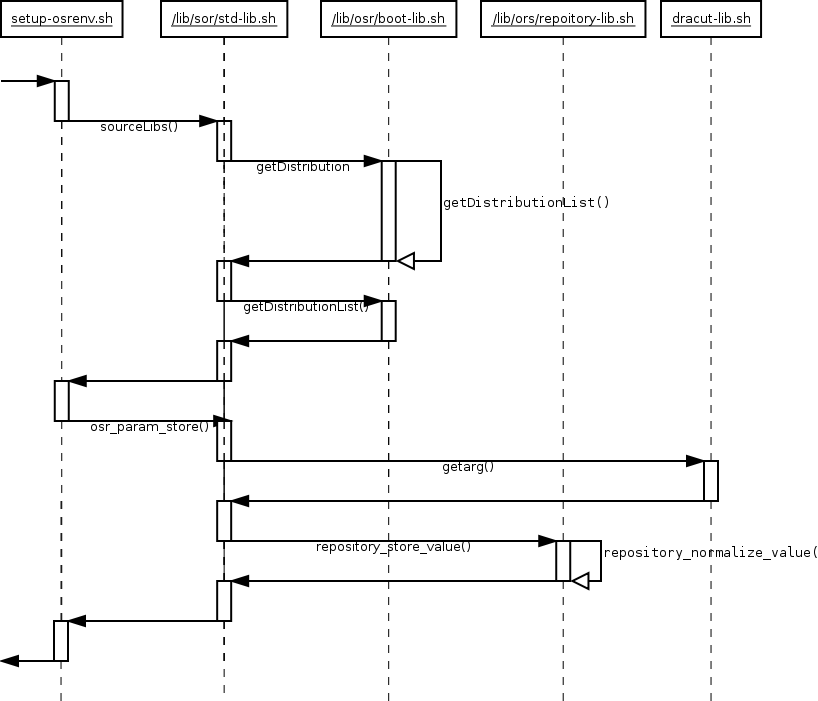
\includegraphics[width=1.0\textwidth,height=1.0\textwidth]{./sequence_diagram_setup-osrenv_DE_de.png}
 \caption[]{Sequence-Diagram des setup-osrenv.sh-Scrips}
\end{figure}

Das Script lädt \texttt{dracut-lib.sh} und die \texttt{/osr/std-lib.sh}. Das Script versucht herauszufinden um welche Distribution es sich handelt. Und legt dann eine einfache Datenbank  mit Schlüssel-Werte-Paaren an. Die Schlüssel der gespeicherte Werte sind:
\medskip 

\begin{tabular}{|l|l|}
 \hline
\textbf{Name} & \textbf{ Wert} \\ \hline
logofile          & \verb|"/etc/atix-logo.txt"|  \\ \hline
shellrcfile       & \verb|${libdir}/shinitrc|  \\ \hline
shellissue        & \verb|${predir}/etc/issue|  \\ \hline
shellissuetmp     & \verb|${predir}/tmp/issue|  \\ \hline
shell             & \verb|"/bin/bash --rcfile $(repository_get_value shellrcfile)"|  \\ \hline
sysctlfile        & \verb|"${predir}/etc/sysctl.conf"|  \\ \hline
xtabfile          & \verb|/etc/xtab|  \\ \hline
xrootfsfile       & \verb|/etc/xrootfs|  \\ \hline
xkillallprocsfile & \verb|/etc/xkillallprocs|  \\ \hline
\end{tabular} 


\subsubsection{parse-nodeid.sh}
\begin{description}
\item[Hook:] cmdline
\item[Priorität:] 2
\end{description}

\begin{figure}[H]
 \centering
 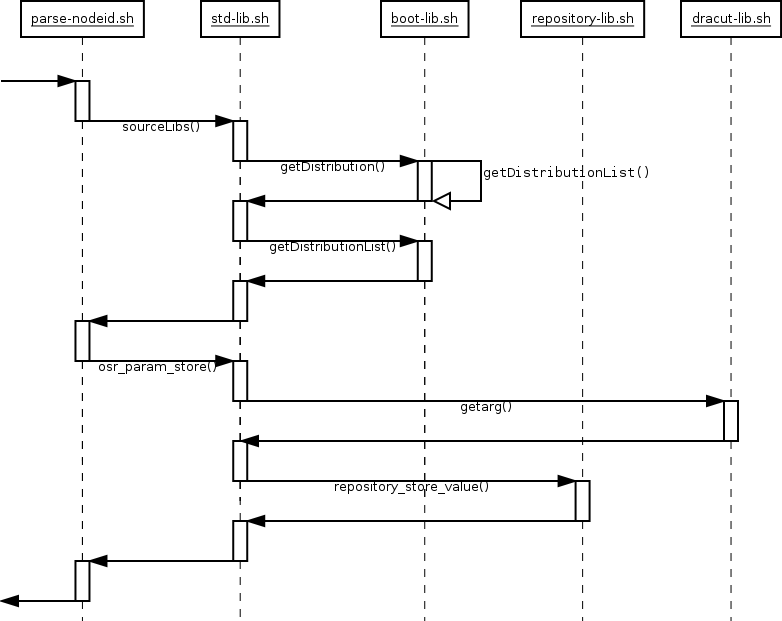
\includegraphics[width=1.0\textwidth,height=1.0\textwidth]{./sequence_diagram_parse-nodeid_DE_de.png}
 \caption[]{Sequence-Diagram des parse-nodeid.sh-Scrips}
\end{figure}

Das Script überprüft noch ein mal die Art der Distribution und speichert den Namen in eine einfache Schlüssel-Werte-Tabelle (mittels der Funktion \texttt{repository\_store\_value()} aus der Datei  \texttt{repository-lib.sh})
Das Script überprüft ob den Kernel die Node-ID als Parameter übergeben wurde.


\subsubsection{parse-cdsl.sh}
\begin{description}
\item[Hook:] cmdline
\item[Priorität:] 99
\end{description}

Das Scrip legt in eine einfache Datenbank mit Schlüssel-Werte-Paaren an. Die Schlüssel der gespeicherte Werte sind:

\medskip 

\begin{tabular}{|l|l|}
 \hline
\textbf{Name} & \textbf{ Wert} \\ \hline
cdsltree & /cluster/cdsl \\ \hline
cdslsharedtree & /cluster/shared \\ \hline
cdsllink & /cdsl.local \\ \hline
\end{tabular} 

\subsubsection{mount-cdsl.sh}
\begin{description}
\item[Hook:] pre-pivot
\item[Priorität:] 1
\end{description}

Das Script macht den --bind-mount für das Chared-Root-File-System. Das wird mit cdsllinks realisiert.

\begin{figure}[H]
 \centering
 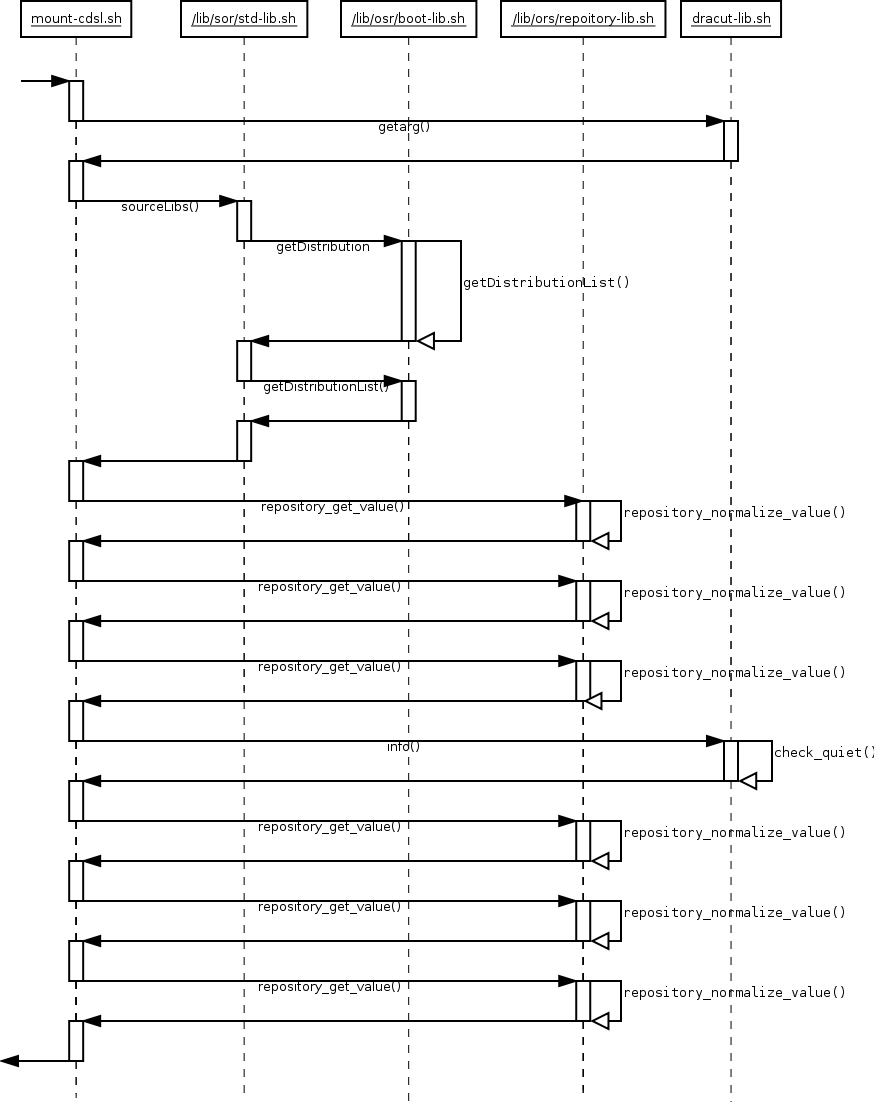
\includegraphics[width=1.0\textwidth,height=1.0\textwidth]{./sequence_diagram_mount-cdsl_DE_de.png}
 \caption[]{Sequence-Diagram des mount-cdsl.sh-Script}
\end{figure}


\subsubsection{write-xfiles.sh}
\begin{description}
\item[Hook:] pre-pivot
\item[Priorität:] 90
\end{description}

Je nach verwendeten File-System des des Chared-Root-Tree wird eine bestimmte Lib eingehangen. Dann die /etc/xtab erstellt bzw.  generiert. Dann wird das \texttt{xrootfs} erstellt und der \texttt{xkillall\_procs}.

\begin{figure}[H]
 \centering
 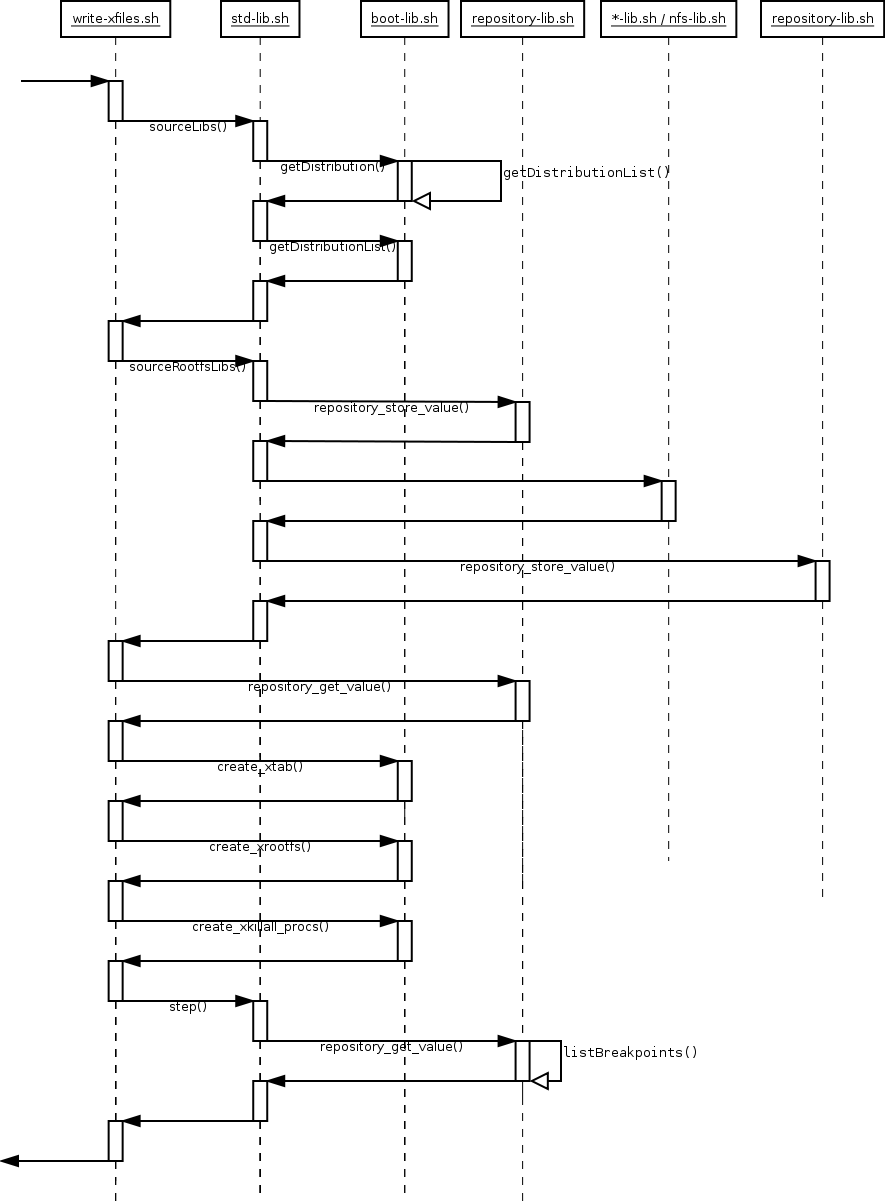
\includegraphics[width=1.0\textwidth,height=1.0\textwidth]{./sequence_diagram_write-xfiles_DE_de.png}
 \caption[]{Sequence-Diagram des write-xfiles.sh-Script}
\end{figure}

\subsubsection{emergencyenv.sh}
\begin{description}
\item[Hook:] emergency
\item[Priorität:] 1
\end{description}

Das Script sorgt für ein Semigraphische Login-Graphik. Dies geschieht durch das setzen der ENV-Variable auf das Script /sbin/shinit.sh.

\section{Modul 99osr-atix-legacy}

Das Modul stellt lediglich ein Semigrafisches Logo zur Verfügung, was dem User beim Login gezeigt wird.




\section{Quellen- und Literaturangaben}
\label{sec:quell}

\begin{itemize}
 \item fedora-Projekt: \url{http://fedoraproject.org/wiki/Dracut}
 \item Projektseite: \url{https://dracut.wiki.kernel.org/}
 \item News: \url{http://git.kernel.org/?p=boot/dracut/dracut.git;a=blob_plain;f=NEWS}
\end{itemize}





\end{document}